\section{Results}\label{sec:results}

\subsection{Modalities, fusion and cost (RQ1)}

Table~\ref{tab:cost} lists the measured cost of each processing step. Face detection and frame decoding (0.51\,s per clip) cost more than the cheap visual model itself. The CLIP image encoder is the most expensive component (0.88\,s), followed by wav2vec~2.0 (0.39\,s). Running all four extractors costs 2.01\,CPU-seconds per clip, a real-time factor of 0.54 on two threads. One CPU core pair can therefore analyse slightly less than two streams in real time.

\begin{table}[t]
\caption{Measured CPU cost per clip (seconds; mean over 1380 clips, two threads). RTF: real-time factor, compute time divided by clip duration.}\label{tab:cost}
\centering\footnotesize
\begin{tabular}{@{}lrrr@{}}
\toprule
Component or pipeline & Mean (SD) & Median & RTF \\
\midrule
Audio decoding & 0.090 (0.018) & 0.085 & 0.025 \\
Video decoding and face detection & 0.512 (0.127) & 0.485 & 0.139 \\
A0 prosody & 0.072 (0.081) & 0.068 & 0.020 \\
A1 wav2vec 2.0 & 0.393 (0.070) & 0.377 & 0.107 \\
V0 MobileNetV3 & 0.065 (0.030) & 0.057 & 0.018 \\
V1 CLIP ViT-B/32 & 0.877 (0.177) & 0.842 & 0.237 \\
\midrule
A1 alone (incl.\ decoding) & 0.483 (0.074) & 0.466 & 0.131 \\
Cheap stage A0+V0 (incl.\ decoding) & 0.738 (0.164) & 0.714 & 0.201 \\
All four models (F-all) & 2.008 (0.320) & 1.964 & 0.545 \\
\botrule
\end{tabular}
\end{table}

Table~\ref{tab:main} reports subject-independent recognition. Chance level is 12.5\% for eight balanced classes (13.3\% for the majority class). The self-supervised speech model is the strongest single modality (72.1\% accuracy), well ahead of CLIP image features (59.9\%) and of the cheap prosody and MobileNet features (both about 48\%). Within wav2vec~2.0 the most informative single layer was layer 3 (71.2\%; Fig.~\ref{fig:layers} in the appendix). Averaging all layers was slightly better (72.1\%) and avoids a layer search. Zero-shot CLIP reached only 20.0\%. It barely exceeds chance. It labelled 61\% of all clips as neutral, including 178 of the 192 happy clips, and most of the rest as angry. A general-purpose vision--language model therefore does not recognise acted facial affect from text prompts alone, although its image features carry the information once a light classifier is trained on them.

Fusion gave the largest gain. Late fusion of the two expensive models (F-full) reaches 82.5\% and fusion of all four (F-all) 82.6\%. This is 10.5 percentage points above the best single modality (Wilcoxon over 24 actors, $p=0.0001$). Adding the cheap models to F-full brings no further gain ($p=0.73$). Early fusion by concatenating A1 and V1 features is worse than late fusion (79.1\%), in line with observations that jointly fitted multimodal classifiers can underuse the weaker modality \citep{wang2020}. A confidence-weighted variant of late fusion (CWF) did not improve on the plain product rule on clean data (81.9\%). Figure~\ref{fig:confusion} in the appendix shows the confusion matrix of F-all. Sad is the hardest class (recall 0.68) and is mostly confused with neutral, calm and fearful. Angry is the easiest (0.90).

\begin{table}[t]
\caption{Subject-independent recognition on RAVDESS (1440 clips, 24 actors, six folds). 95\% CIs from a cluster bootstrap over actors. Cost: mean CPU seconds per clip.}\label{tab:main}
\centering\footnotesize
\begin{tabular}{@{}lccr@{}}
\toprule
System & Accuracy [95\% CI] & Macro-F1 [95\% CI] & Cost \\
\midrule
A0 prosody & 0.477 [0.436, 0.519] & 0.465 [0.423, 0.505] & 0.16 \\
A1 wav2vec 2.0 & 0.721 [0.678, 0.758] & 0.715 [0.676, 0.752] & 0.48 \\
V0 MobileNetV3 & 0.476 [0.412, 0.540] & 0.473 [0.410, 0.536] & 0.58 \\
V1 CLIP & 0.599 [0.560, 0.642] & 0.592 [0.552, 0.636] & 1.39 \\
V1-ZS CLIP zero-shot & 0.200 [0.171, 0.229] & 0.161 [0.126, 0.193] & 1.39 \\
\midrule
F-cheap: LF(A0, V0) & 0.626 [0.569, 0.687] & 0.618 [0.561, 0.679] & 0.74 \\
EF-full: concat(A1, V1) & 0.791 [0.749, 0.832] & 0.786 [0.744, 0.826] & 1.87 \\
F-full: LF(A1, V1) & 0.825 [0.785, 0.861] & 0.821 [0.779, 0.858] & 1.87 \\
F-all: LF(A0, A1, V0, V1) & \textbf{0.826} [0.778, 0.870] & \textbf{0.822} [0.773, 0.867] & 2.01 \\
\midrule
Cascade, stage 1 = A0+V0 & 0.815 [0.762, 0.862] & 0.811 [0.760, 0.859] & 1.65 \\
Cascade, stage 1 = A1 & 0.800 [0.752, 0.843] & 0.796 [0.749, 0.839] & 1.05 \\
\botrule
\end{tabular}
\end{table}

\subsection{Cost-aware cascades (RQ2)}

Figure~\ref{fig:cascades} plots accuracy against mean cost for cascades with different first stages, sweeping the escalation rate from 0 to 100\%. At every escalation rate except one, every cascade was at least as accurate as escalating a random subset of the same size. The exception was the A0+V0 cascade at 2\% escalation, where it was 0.1 points worse. For example, the A0+V0 cascade at 40\% escalation reaches 76.3\% compared with 70.6\% for random escalation. Stage-1 confidence is therefore informative on clean data. The choice of first stage matters more than the threshold. Our initial design (Cycle~1) used the two cheapest models, A0+V0, as stage 1. It is dominated across almost the whole cost range by the cascade that starts with the speech transformer A1, because A1 alone is both cheaper (0.48\,s) and much more accurate (72.1\% vs 62.6\%) than A0+V0. The visual pipeline is expensive in our setting because face detection and decoding cost 0.51\,s before any visual model runs.

\begin{figure}[t]
\centering
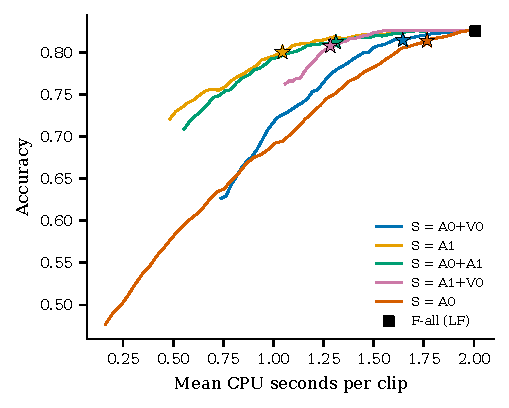
\includegraphics[width=0.62\textwidth]{figures/cascade_orders.pdf}
\caption{Accuracy against mean CPU cost per clip for confidence-gated cascades with different first stages $S$, each escalating to F-all. Curves sweep the escalation rate. Stars mark the operating points chosen on training data only.}\label{fig:cascades}
\end{figure}

Table~\ref{tab:orders} gives the operating points fixed on training data. All cascades lose between 1.1 and 2.6 points of accuracy relative to F-all on the test people, more than the one-point tolerance targeted on training data. Thresholds tuned on one set of people did not carry over exactly to new people. The A1-first cascade escalates 37\% of clips and saves 47.9\% of compute at a loss of 2.6 points (80.0\% vs 82.6\%; Holm-adjusted $p=0.038$). The A0+A1 cascade saves 34.7\% at a loss of 1.4 points that is not significant after correction. The Cycle~1 design (A0+V0) saves only 18.0\%. On the test sweep, the A1-first cascade reaches 82\% accuracy at 1.43\,s per clip, 29\% cheaper than F-all. This value is chosen on the test data and is therefore optimistic. To check that the choice of first stage does not depend on test data, we repeated the selection inside each outer fold. Each candidate's operating point and mean cost were estimated on out-of-fold training predictions, and the cheapest candidate was chosen. A1 was chosen in all six folds, so the nested procedure reproduces the A1 row of Table~\ref{tab:orders}. In every fold, test accuracy was again below that of F-all.

\begin{table}[t]
\caption{Cascade operating points fixed on training data and applied to held-out actors. Saving relative to F-all (2.008\,s per clip, accuracy 0.826). $p$: Wilcoxon test of per-actor accuracy against F-all, Holm-adjusted over the eight first stages.}\label{tab:orders}
\centering\footnotesize
\begin{tabular}{@{}lrrrrrr@{}}
\toprule
Stage 1 & Stage-1 cost & Escalation & Mean cost & Saving & Accuracy & $p_\text{Holm}$ \\
\midrule
A0 & 0.162 & 0.869 & 1.767 & 12.0\% & 0.814 & 0.061 \\
V0 & 0.576 & 0.866 & 1.816 & 9.6\% & 0.803 & 0.270 \\
A0+V0 (Cycle 1) & 0.738 & 0.715 & 1.645 & 18.0\% & 0.815 & 0.061 \\
A1 & 0.483 & 0.369 & 1.045 & 47.9\% & 0.800 & 0.038 \\
A0+A1 & 0.555 & 0.521 & 1.312 & 34.7\% & 0.812 & 0.105 \\
A1+V0 & 1.059 & 0.237 & 1.284 & 36.1\% & 0.808 & 0.041 \\
A0+A1+V0 & 1.131 & 0.309 & 1.402 & 30.2\% & 0.810 & 0.105 \\
V1 & 1.388 & 0.764 & 1.861 & 7.3\% & 0.808 & 0.105 \\
\botrule
\end{tabular}
\end{table}

\subsection{Stream degradations and the silent-failure problem (RQ3)}

Table~\ref{tab:robust} shows what happens when the stream degrades. Audio noise is severe. Accuracy of wav2vec~2.0 drops from 72.1\% to 50.3\% at 20\,dB and to 16.9\% at 0\,dB, close to chance. Visual impairments roughly halve CLIP accuracy (compress 34.3\%, blur 32.5\%, low light 46.2\%). Because late fusion combines evidence, a degraded channel pulls the fused decision down even when the other channel is intact. At 0\,dB, F-all (17.8\%) is far worse than the clean visual models alone (59.9\% for CLIP).

\begin{table}[t]
\caption{Accuracy under stream degradations (models trained on clean data). Conf.: mean stage-1 confidence of the A0+V0 stage. Esc.: escalation rate of the Cycle~1 cascade at its fixed threshold.}\label{tab:robust}
\centering\footnotesize
\begin{tabular}{@{}lrrrrrrr@{}}
\toprule
Condition & A1 & V1 & F-cheap & Conf. & F-all & Cascade & Esc. \\
\midrule
clean & 0.721 & 0.599 & 0.626 & 0.635 & 0.826 & 0.815 & 0.715 \\
snr20 & 0.503 & 0.599 & 0.351 & 0.714 & 0.622 & 0.560 & 0.578 \\
snr10 & 0.325 & 0.599 & 0.245 & 0.816 & 0.370 & 0.306 & 0.367 \\
snr0 & 0.169 & 0.599 & 0.180 & 0.907 & 0.178 & 0.178 & 0.171 \\
compress & 0.721 & 0.343 & -- & -- & 0.702 & 0.674 & 0.726 \\
lowlight & 0.721 & 0.462 & -- & -- & 0.684 & 0.651 & 0.673 \\
blur & 0.721 & 0.325 & -- & -- & 0.734 & 0.711 & 0.749 \\
snr10+compress & 0.325 & 0.343 & -- & -- & 0.360 & 0.333 & 0.564 \\
snr0+lowlight & 0.169 & 0.462 & -- & -- & 0.166 & 0.162 & 0.284 \\
\botrule
\end{tabular}
\end{table}

The confidence column of Table~\ref{tab:robust} shows the main result of Cycle~1. As audio noise increases, the accuracy of the cheap stage falls from 62.6\% to 18.0\%, but its mean confidence \emph{rises} from 0.64 to 0.91. A plausible explanation, which we did not test directly, is that noise moves the inputs far from the training data, where linear classifiers extrapolate to extreme and therefore confident scores. Over-confidence under distribution shift is well documented for neural classifiers \citep{ovadia2019}. Our result shows that it also occurs in a multimodal affect pipeline, and that it defeats the two mechanisms that depend on confidence. The cascade reads high confidence as ``easy'' and escalates less: 72\% of clips on clean data, 37\% at 10\,dB and 17\% at 0\,dB. It therefore saves the most compute exactly when its answers are worst. Figure~\ref{fig:silent} shows one such stream. The pattern is not limited to the cheap stage. The confidence of the audio-only fusion LF(A0, A1) rose from 0.80 to 0.995 at 0\,dB while its accuracy fell from 70.9\% to 13.5\%. The confidence of F-all rose from 0.89 to 0.97 while its accuracy fell to 17.8\%. Temperature scaling, fitted on clean training data, lowered the level of confidence but did not change this pattern (F-all ECE 0.023 clean, 0.756 at 0\,dB). Confidence-weighted fusion, which weights each modality by one minus the normalised entropy of its posterior, fails for the same reason. It was significantly worse than plain late fusion under 10 and 0\,dB noise and in both combined conditions (e.g.\ 31.9\% vs 37.0\% at 10\,dB; Holm-adjusted $p=0.0005$). Under the visual impairments, where confidence did not rise, it was slightly better (not significant).

\begin{figure}[t]
\centering
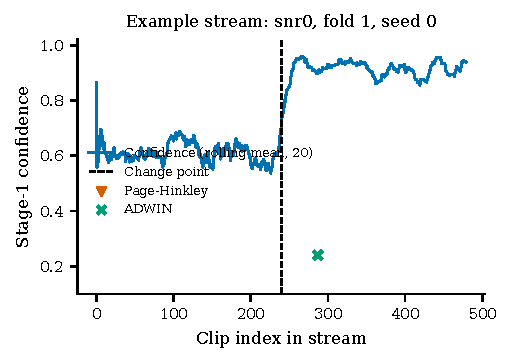
\includegraphics[width=0.55\textwidth]{figures/drift_stream.pdf}
\caption{A silent failure. Rolling mean of stage-1 confidence on a stream of 240 clean clips followed by 240 clips with 0\,dB audio noise (fold 1, seed 0). Accuracy collapses after the change point while confidence rises. A one-sided Page--Hinkley test that watches for falling confidence stays silent. A two-sided ADWIN detector fires only after the confidence jump has persisted for several dozen clips.}\label{fig:silent}
\end{figure}

This failure carries over to label-free drift monitoring (Table~\ref{tab:drift}). A Page--Hinkley test that looks for falling confidence, the usual alarm for a model in trouble, did not detect any of the audio-only noise conditions. It detected only 35\% of the compressed and 72\% of the blurred streams. A two-sided ADWIN detector on confidence noticed the jump at 0\,dB but detected only 17\% of the 20\,dB streams and none of the visual degradations. In those conditions the cheap stage's confidence changes too little to separate from normal variation. Confidence also gives no hint of which channel is at fault.

The per-channel input monitors behave very differently. Figure~\ref{fig:monitors} shows their scores. The distribution of each monitor's score moves upwards under every impairment of its own channel, while clean clips of new people stay below the threshold. With ADWIN on the standardised monitor scores, every degradation was detected in all 120 streams. The median delay was 15 clips (about 55\,s of speech) in seven conditions and 47 clips for blur. In the gating analyses below a channel's state changes from the next clip, so the same alarms appear there as delays of 16 and 48 clips. In every single-channel condition the first alarm came from the degraded channel (Table~\ref{tab:drift}). In the combined conditions both channels are degraded, so any first alarm counts as correct. On the clean control streams the monitors raised no false alarm. These streams replay the 240 clean test clips of a fold in two random orders, so they show that the detector does not fire on random variation among clean clips. They are weaker evidence about natural shifts such as a change of speaker. We therefore also presented the clean test clips grouped by speaker, so that the stream changes speaker every 60 clips. Here the monitors did fire. At least one channel was marked as degraded in 69\% of these streams (1.9 marks per 1000 clips), and stream-level gating then removed a healthy channel for 21\% of the clips. Accuracy fell from 82.6\% to 79.3\%. The monitors compare each clip with the population of training speakers, so a new speaker whose voice or face lies at the edge of that population looks like a shift. Section~\ref{sec:cycle5} tests two remedies. River's ADWIN implementation tests for change every 32 observations. Together with the change point at clip 240, this quantises the delays to 15 or 47 clips. Faster detection is possible by checking more often, at the price of more tests. A Page--Hinkley test on the same scores works as well once its threshold is set for the scale of the signal. With the threshold used for the confidence signal ($\lambda=5$) it produced 17--21 false alarms per 1000 clean clips. At $\lambda=40$ it produced fewer than 0.1 false alarms per 1000 clips and detected every single-channel degradation after 10--21 clips. The input signal matters more than the choice of detector, while ADWIN needed no tuning.

\begin{table}[t]
\setlength{\tabcolsep}{4pt}
\caption{Label-free drift detection, 120 streams per condition (240 clean clips, then 240 degraded). Det.: share of streams with an alarm after the change. Delay: median clips after the change (IQR). Attr.: share of streams whose first alarm comes from the degraded channel. False alarms per 1000 clips of clean control streams: confidence-PH 0.47, confidence-ADWIN 0, input-monitor ADWIN 0.}\label{tab:drift}
\centering\footnotesize
\begin{tabular}{@{}lrrrrrr@{}}
\toprule
 & \multicolumn{1}{c}{Confidence, PH} & \multicolumn{2}{c}{Confidence, ADWIN} & \multicolumn{3}{c}{Input monitors, ADWIN} \\
\cmidrule(lr){2-2}\cmidrule(lr){3-4}\cmidrule(l){5-7}
Condition & Det. & Det. & Delay & Det. & Delay & Attr. \\
\midrule
snr20 & 0.00 & 0.17 & 175 (175--207) & 1.00 & 15 (15--47) & 1.00 \\
snr10 & 0.00 & 0.70 & 111 (79--143) & 1.00 & 15 (15--15) & 1.00 \\
snr0 & 0.00 & 1.00 & 79 (79--79) & 1.00 & 15 (15--15) & 1.00 \\
compress & 0.35 & 0.00 & -- & 1.00 & 15 (15--15) & 1.00 \\
lowlight & 0.00 & 0.00 & -- & 1.00 & 15 (15--15) & 1.00 \\
blur & 0.72 & 0.00 & -- & 1.00 & 47 (15--47) & 1.00 \\
snr10+compress & 0.02 & 0.02 & 239 & 1.00 & 15 (15--15) & 1.00 \\
snr0+lowlight & 0.00 & 0.88 & 79 (79--111) & 1.00 & 15 (15--15) & 1.00 \\
\botrule
\end{tabular}
\end{table}

\begin{figure}[t]
\centering
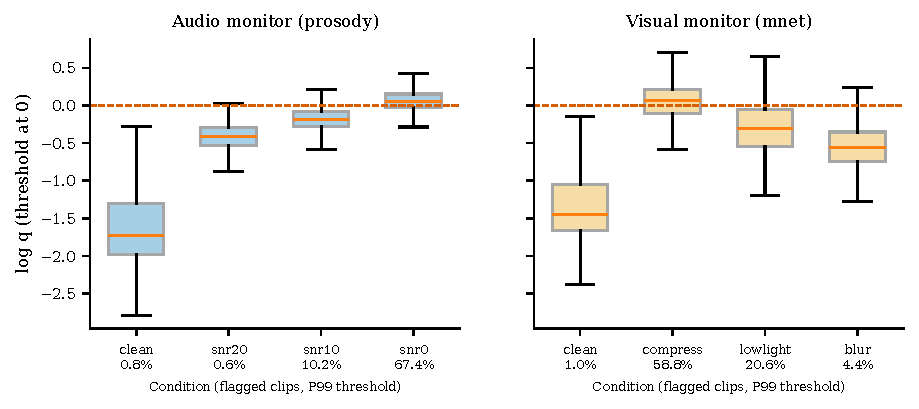
\includegraphics[width=\textwidth]{figures/monitor_scores.pdf}
\caption{Scores of the label-free input monitors on held-out actors (log of normalised Mahalanobis distance; 0 is the per-clip threshold). Percentages give the share of clips above the threshold. Each monitor's score shifts under every impairment of its channel. Under moderate degradation most clips stay below the per-clip threshold, but the shift in the mean is easy to detect at stream level.}\label{fig:monitors}
\end{figure}

\subsection{From monitoring to action: gating (RQ4, Cycles 2 and 3)}

Cycle~2 used the monitors clip by clip. A clip whose channel score exceeded the threshold was fused without that channel. Figure~\ref{fig:monitors} explains why this was only partly successful. At 0\,dB, 67\% of clips are flagged and clip-level gating raised F-all accuracy from 17.8\% to 46.5\% (24 of 24 actors improved; Holm-adjusted $p=0.0002$). At 10\,dB only 10\% of clips are flagged and the gain was small and not significant (37.0\% to 40.1\%). In the combined snr10+compress condition the visual monitor flagged 59\% of clips while the audio monitor flagged only 10\%. The policy then removed the still-informative visual channel and kept the noisy audio, and accuracy fell from 36.0\% to 27.1\% (Holm-adjusted $p=0.003$). The gains also depended on the threshold. At the 99.9th percentile the audio monitor flagged only 1\% of 0\,dB clips and the benefit disappeared. Clip-level gating is therefore fragile, because a per-clip test has to separate distributions that overlap heavily.

Cycle~3 acts on the stream-level detector instead (Algorithm~\ref{alg:slg}). Table~\ref{tab:gating} compares the gating policies on the degraded segment of the simulated streams. The oracle drops the truly degraded channel immediately. Stream-level gating raised accuracy under 10\,dB noise from 37.0\% to 60.3\% and under 0\,dB noise from 17.8\% to 59.3\%, close to the oracle's 62.2\%. Both gains were significant across actors (Holm-adjusted $p<10^{-4}$). The remaining gap to the oracle is the detection delay, during which clips are still fused with the noisy channel. For the visual impairments, stream-level gating was within $\pm2.3$ points of plain fusion, and no difference was significant. When video is compressed, dark or blurred but the voice is clean, there is little to gain from dropping the visual channel, and for blur the degraded video still adds information (oracle 70.9\% vs plain fusion 73.4\%). In both combined conditions both channels were flagged at almost the same time. With no healthy channel left, the policy fell back to full fusion. It did no harm, but the gain was at most marginal (+0.8 points at snr0+lowlight). In that case the system should alert an operator. On clean control streams the policy never gated a channel. Its accuracy was identical to plain fusion, and its overhead was the monitor computation (about 0.6\,ms per clip). Because the expensive model of a degraded channel is skipped, gating also reduced cost. Over the degraded segment alone it fell to 1.64--1.66\,s per clip under audio noise and to 1.19--1.26\,s under visual impairments.

\begin{table}[t]
\caption{Accuracy on the degraded part of the simulated streams (240 clean clips followed by 240 degraded; 6 folds $\times$ 20 seeds). LF: plain fusion of all models. Clip: clip-level gating (Cycle~2). Stream: stream-level gating (Cycle~3). Oracle: the truly degraded channel is dropped at the change point. Cost: mean CPU seconds per clip for stream-level gating over the whole stream, half of which is clean. $p$: Wilcoxon, stream-level gating vs LF over 24 actors, Holm-adjusted.}\label{tab:gating}
\centering\footnotesize
\begin{tabular}{@{}lrrrrrr@{}}
\toprule
Condition & LF & Clip & Stream & Oracle & Cost & $p_\text{Holm}$ \\
\midrule
snr20 & 0.622 & 0.617 & 0.621 & 0.622 & 1.83 & 1.000 \\
snr10 & 0.370 & 0.401 & \textbf{0.603} & 0.622 & 1.83 & $<$0.001 \\
snr0 & 0.178 & 0.465 & \textbf{0.593} & 0.622 & 1.82 & $<$0.001 \\
compress & 0.702 & 0.716 & 0.709 & 0.709 & 1.60 & 1.000 \\
lowlight & 0.684 & 0.699 & 0.706 & 0.709 & 1.61 & 1.000 \\
blur & 0.734 & 0.729 & 0.715 & 0.709 & 1.63 & 1.000 \\
snr10+compress & 0.360 & 0.271 & 0.360 & 0.360 & 2.01 & 1.000 \\
snr0+lowlight & 0.166 & 0.249 & 0.174 & 0.166 & 2.00 & 0.013 \\
\botrule
\end{tabular}
\end{table}

Figure~\ref{fig:slg} shows the policy on streams that degrade and then recover. In the recovery scenario every degradation was detected in all streams. The degraded channel was re-enabled after the stream returned to clean in 96--100\% of streams, with a median delay of 32 clips. Until then the system runs without the channel, so accuracy on the final clean segment was 78--80\% instead of 82--83\% when one channel had been degraded. It was unaffected after the combined conditions, where no channel had been dropped. Operators will need to tune the recovery delay. Re-enabling a channel faster than it was disabled is one option.

\begin{figure}[t]
\centering
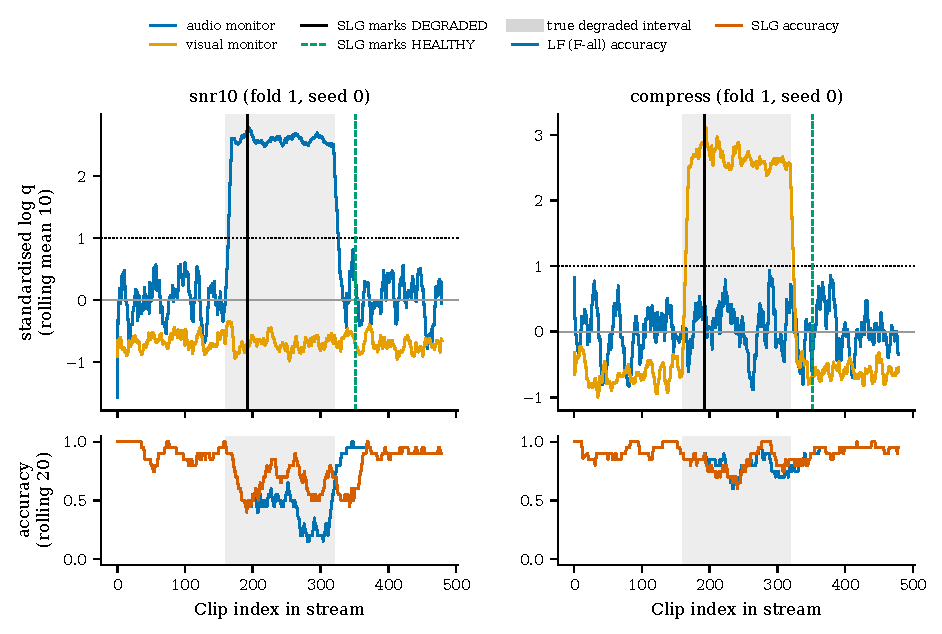
\includegraphics[width=\textwidth]{figures/slg_stream.pdf}
\caption{Stream-level gating on streams that degrade and recover (160 clean, 160 degraded, 160 clean clips; fold 1, seed 0). Upper panels: standardised input-monitor scores per channel (rolling mean) with the true degraded interval shaded and the gating decisions marked. Lower panels: rolling accuracy of plain fusion and stream-level gating. Left: 10\,dB audio noise. Right: video compression.}\label{fig:slg}
\end{figure}

\subsection{Robust training and envelope-aware gating (Cycle 4)}

All results so far used models trained on clean data. A standard alternative is multi-condition training (MCT), which trains on degraded copies of the training data. We retrained each modality model on clean data together with one degraded copy (audio models: 10\,dB noise; visual models: compression). Everything else was unchanged, including subject-independent folds and calibration on out-of-fold predictions. Table~\ref{tab:mct} shows that MCT is by far the strongest single lever for robustness. On clean data it was as accurate as clean training (83.1\% vs 82.6\%; $p=0.95$ after Holm correction). Under the two conditions seen in training it recovered almost all of the loss (10\,dB: 80.6\% vs 37.0\%; compression: 80.3\% vs 70.2\%). It also generalised to unseen noise levels (20\,dB: 79.7\%; 0\,dB: 59.7\%) and to the combined conditions. The exception was low light, which MCT did not help (67.8\% vs 68.4\%). After MCT the fused model no longer became more confident under noise (mean confidence 0.90 clean, 0.82 at 0\,dB). Its calibration still deteriorated, though: the gap between confidence and accuracy grew from 7 points on clean data to 23 points at 0\,dB.

\begin{table}[t]
\caption{Accuracy of F-all on the degraded part of the simulated streams for clean training and multi-condition training (MCT), with and without stream-level gating. Gating uses either monitors fitted on clean data (clean-fit) or monitors fitted on the multi-condition training data (envelope). $\dagger$: condition seen in MCT training. $p$: Wilcoxon over 24 actors, Holm-adjusted over 8 conditions; * $p<0.05$ for the comparison with MCT without gating.}\label{tab:mct}
\centering\footnotesize
\begin{tabular}{@{}lrrrrr@{}}
\toprule
 & \multicolumn{2}{c}{Clean training} & \multicolumn{3}{c}{Multi-condition training} \\
\cmidrule(lr){2-3}\cmidrule(l){4-6}
Condition & No gating & Clean-fit gating & No gating & Clean-fit gating & Envelope gating \\
\midrule
snr20 & 0.622 & 0.621 & 0.797 & 0.628* & 0.797 \\
snr10$^\dagger$ & 0.370 & 0.603 & 0.806 & 0.619* & 0.806 \\
snr0 & 0.178 & 0.593 & 0.597 & 0.605 & 0.597 \\
compress$^\dagger$ & 0.702 & 0.709 & 0.803 & 0.712* & 0.803 \\
lowlight & 0.684 & 0.706 & 0.678 & 0.703 & 0.703 \\
blur & 0.734 & 0.715 & 0.769 & 0.717* & 0.766 \\
snr10+compress$^\dagger$ & 0.360 & 0.360 & 0.789 & 0.789 & 0.789 \\
snr0+lowlight & 0.166 & 0.174 & 0.420 & 0.419 & 0.393 \\
\botrule
\end{tabular}
\end{table}

MCT changes the role of gating. With MCT models, gating driven by the clean-fit monitors was harmful. It lowered accuracy significantly under 20 and 10\,dB noise (by 17 and 19 points), compression (9 points) and blur (5 points). The monitors correctly detected that the inputs differed from clean data, but the robust models could still use the degraded channel, and dropping it threw that information away. Gating should therefore respond to shifts outside the conditions the models were trained for, the \emph{training envelope}, and not to any departure from clean data. In Cycle~4 we kept the clean-fit monitors for alerting and diagnosis and added a second pair of monitors fitted on the multi-condition training features, which drive gating. Envelope-aware gating never fired on the conditions inside the envelope and so did no harm there. It fired on low light (detected in all streams), where it raised accuracy from 67.8\% to 70.3\% (not significant), and rarely on blur. It did not fire on 0\,dB noise. A possible reason, which we did not test, is that a reference distribution fitted on clean and 10\,dB audio is wide enough to absorb 0\,dB noise along the same directions. In the combined snr0+lowlight condition it fired on the visual channel and lowered accuracy by 2.7 points (not significant). Inside the training envelope envelope-aware gating is a safe default, but in our conditions it adds little to MCT (Fig.~\ref{fig:envelope}). MCT also leaves the cascade intact: an A1-first cascade with MCT models saved 47.4\% of compute at 80.6\% clean accuracy, and under noise it escalated more, not less (44--59\% of clips). The clean-fit monitors remain the source of alerts and attribution. They detected all eight degradations under MCT exactly as before, because they do not depend on the classifiers.

\begin{figure}[t]
\centering
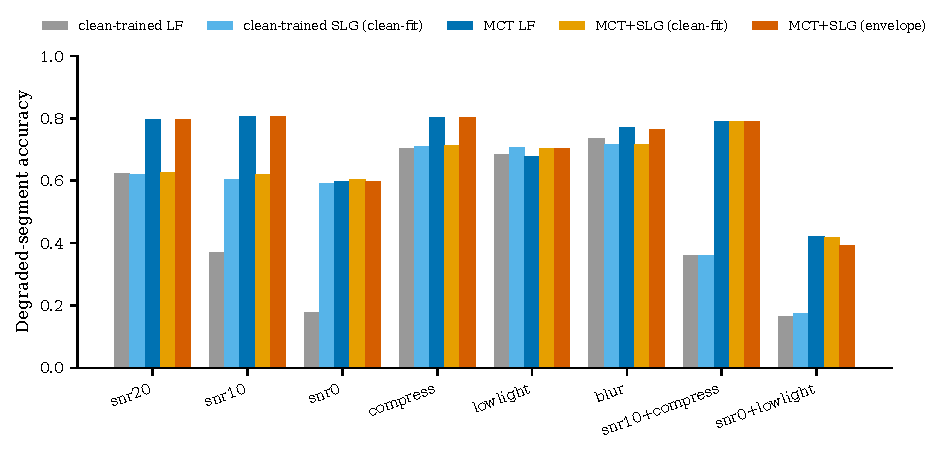
\includegraphics[width=\textwidth]{figures/envelope.pdf}
\caption{Accuracy on the degraded part of the simulated streams for clean-trained and multi-condition-trained (MCT) models, with and without stream-level gating.}\label{fig:envelope}
\end{figure}

\subsection{End-to-end evaluation of the integrated artifact}

The analyses above evaluate cost and robustness separately. Running the monitors has a cost of its own, because the visual monitor needs decoded video and face crops, which the audio-first cascade avoids for most clips. We therefore simulated two integrated variants on the same streams (Table~\ref{tab:integrated}, Fig.~\ref{fig:integrated}). Both use the clean-trained models, a stage~1 of LF(A0,A1) with a recalibrated threshold, escalation to all four models, and stream-level gating. When audio is flagged, clips are routed to the visual models. When video is flagged, the system stays on audio. When both are flagged, outputs are marked as unreliable. Variant IS-B computes the visual monitor on every clip. Variant IS-A computes it only on clips that are escalated anyway, plus every eighth clip while video is flagged.

\begin{table}[t]
\caption{End-to-end evaluation of the integrated artifact on simulated streams (6 folds $\times$ 20 seeds). Accuracy and mean CPU seconds per clip on clean control streams and on the degraded segment. IS-A: visual monitor only on escalated clips; IS-B: visual monitor on every clip.}\label{tab:integrated}
\centering\footnotesize
\begin{tabular}{@{}lrrrrrr@{}}
\toprule
 & \multicolumn{2}{c}{Clean stream} & \multicolumn{2}{c}{snr10 (degraded)} & \multicolumn{2}{c}{compress (degraded)} \\
\cmidrule(lr){2-3}\cmidrule(lr){4-5}\cmidrule(l){6-7}
System & Acc. & Cost & Acc. & Cost & Acc. & Cost \\
\midrule
F-all (no monitoring) & 0.826 & 2.01 & 0.370 & 2.01 & 0.702 & 2.01 \\
A1-first cascade (no monitoring) & 0.800 & 1.05 & 0.347 & 1.06 & 0.730 & 1.05 \\
Stream-level gating on F-all & 0.826 & 2.01 & 0.603 & 1.64 & 0.709 & 1.19 \\
Integrated IS-A & 0.811 & 1.32 & 0.596 & 1.56 & 0.708 & 0.75 \\
Integrated IS-B & 0.811 & 1.59 & 0.596 & 1.59 & 0.709 & 1.16 \\
\botrule
\end{tabular}
\end{table}

\begin{figure}[t]
\centering
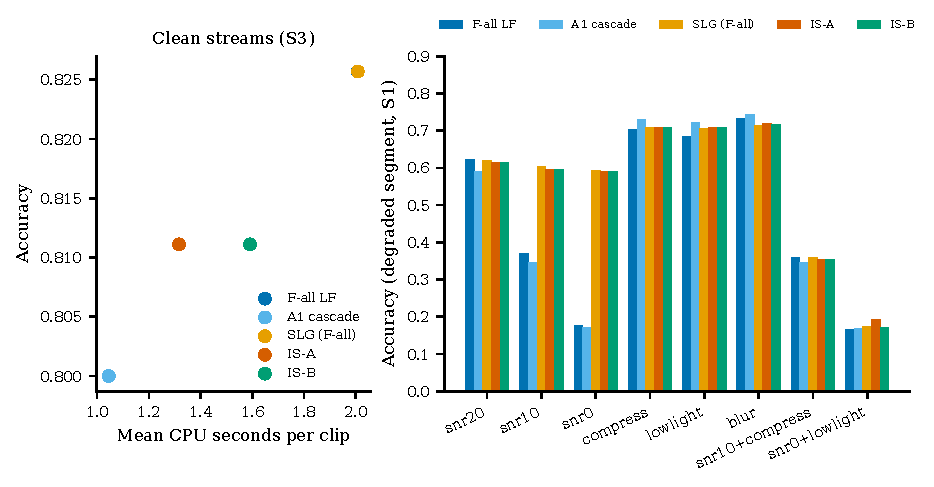
\includegraphics[width=\textwidth]{figures/integrated.pdf}
\caption{End-to-end evaluation. Left: accuracy against mean CPU cost per clip on clean streams. Right: accuracy on the degraded part of the streams for each condition.}\label{fig:integrated}
\end{figure}

On clean streams IS-B cost 1.59\,s per clip, 21\% less than F-all, at 81.1\% accuracy. Under audio noise it kept the robustness of stream-level gating (59.6\% at 10\,dB and 59.0\% at 0\,dB, against 37.0\% and 17.8\% for F-all; Holm-adjusted $p<10^{-4}$). The cheaper IS-A cost 1.32\,s per clip (34\% less than F-all) and behaved like IS-B under audio noise. It failed in one respect. Because the visual monitor saw few clips, single-channel visual degradations were detected later (median 44--71 clips instead of 16--48). After video returned to clean, the visual channel was never re-enabled within the 160-clip recovery window. Accuracy on that final clean segment was 71\% instead of 78--79\% for IS-B. Monitoring has its own cost. A monitor that sees too little of a channel can detect a degradation but miss the moment it ends. The 48\% saving of the unmonitored A1-first cascade (80.0\% accuracy) is therefore an upper bound. With reliable monitoring of both channels, the integrated IS-B saves about 21\% (81.1\% accuracy). On speaker-blocked clean streams the integrated variants lost about 3 points (IS-A 77.7\%, IS-B 78.1\%) because of the alarms on speaker changes, and they abstained on fewer than 0.5\% of clips.

\subsection{Calibration, group parity and explanation (RQ4)}

Product-rule fusion is over-confident. On clean data, F-all had a mean confidence of 0.89 against an accuracy of 0.83 (ECE 0.068). The over-confidence was concentrated in male actors (ECE 0.127 vs 0.028 for female actors). A single temperature per training fold reduced the ECE to 0.023 and closed the calibration gap between the groups (0.047 vs 0.054). Recalibration is not uniformly beneficial, though. For the cheap two-model stage it made calibration for female actors worse (ECE 0.052 to 0.075). Calibration should therefore be checked per group after every recalibration. Accuracy is unchanged because a temperature does not change the ranking of classes.

Accuracy itself differed by group (Table~\ref{tab:fair}). Every system was more accurate for female than for male actors. For F-all the gap was 13.8 points (89.4\% vs 75.7\%), and the 95\% bootstrap interval of the gap, 6.3 to 21.4 points, excludes zero. The gap was larger after fusion than for the best single modality, wav2vec~2.0 (6.4 points, interval including zero). The difference between the two gaps, 7.4 points [1.9, 12.9], excludes zero. Compared with CLIP image features the gap did not differ significantly (3.2 points [$-$6.0, 12.9]). Fusion therefore did not reduce a difference that each modality showed, and relative to the strongest modality it widened it. With 12 actors per group, and actors who differ in expressive style as well as in sex, we cannot attribute the gap to sex as such. The result shows why accuracy should be audited per group before deployment and not inferred from aggregate performance.

\begin{table}[t]
\setlength{\tabcolsep}{4pt}
\caption{Accuracy and calibration by actor sex on clean data. Gap: female minus male accuracy, with 95\% cluster-bootstrap CI. ECE before and after temperature recalibration of the fused output.}\label{tab:fair}
\centering\footnotesize
\begin{tabular}{@{}lrrrrr@{}}
\toprule
System & Acc.\ female & Acc.\ male & Gap [95\% CI] & ECE f/m (raw) & ECE f/m (recal.) \\
\midrule
A1 wav2vec 2.0 & 0.753 & 0.689 & 0.064 [$-$0.007, 0.144] & 0.043 / 0.055 & -- \\
V1 CLIP & 0.651 & 0.546 & 0.106 [0.031, 0.181] & 0.051 / 0.045 & -- \\
F-cheap & 0.678 & 0.575 & 0.103 [$-$0.011, 0.214] & 0.052 / 0.060 & 0.075 / 0.047 \\
F-all & 0.894 & 0.757 & 0.138 [0.063, 0.214] & 0.028 / 0.127 & 0.054 / 0.047 \\
Cascade (A0+V0) & 0.881 & 0.749 & 0.132 [0.050, 0.221] & 0.038 / 0.116 & -- \\
\botrule
\end{tabular}
\end{table}

Late fusion makes each decision decomposable into modality contributions (DR5). For each clip we computed the share of the evidence for the predicted class that came from the audio models (A0, A1) and from the visual models (V0, V1). Figure~\ref{fig:attr} shows the mean shares by true emotion. Audio contributed most of the evidence overall (50--66\%). Its share was highest for surprised (66\%), fearful (64\%) and calm (61\%) and lowest for happy, where face and voice contributed equally. This agrees with the common finding that happiness is the most visually distinctive emotion. Among the prosodic descriptors, the two largest standardised coefficients belonged to the mean and variability of the first cepstral coefficient, which tracks overall energy. Low-order cepstral means and energy (RMS) statistics also ranked in the top ten. These are interpretable loudness and spectral-shape cues associated with arousal. These explanations are coarse, and computing them adds no inference cost. They also tell an operator which channel a decision relied on. This matters when that channel is the one a monitor has just flagged.

\begin{figure}[t]
\centering
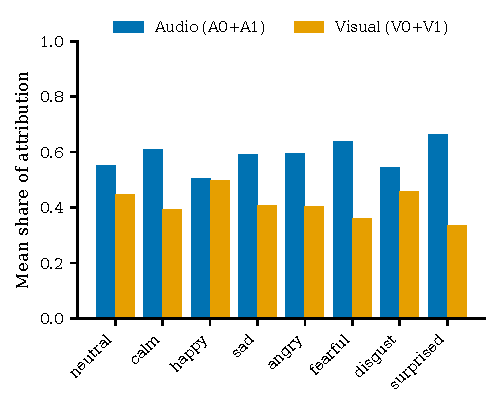
\includegraphics[width=0.55\textwidth]{figures/attribution.pdf}
\caption{Modality attribution for F-all: mean share of the evidence for the predicted class that comes from the audio models (A0+A1) and from the visual models (V0+V1), by true emotion.}\label{fig:attr}
\end{figure}

\subsection{Confirmatory evaluation and quality-descriptor monitors (Cycle 5)}\label{sec:cycle5}

\paragraph{Replication on CREMA-D.} With the design of Cycles~1--4 frozen, the main findings of Cycles~1--4 were replicated on the 91 CREMA-D speakers (Table~\ref{tab:replication}). Over six classes (chance 16.7\%), A1 reached 70.3\%, V1 58.1\%, A0 53.1\% and V0 50.6\%. F-all reached 79.6\% [77.2, 82.0], 9.3 points above A1 (Wilcoxon over 91 actors, Holm-adjusted $p<0.001$). The A1-first cascade, with its operating point fixed on training predictions, reached 78.3\% at 1.10\,s of CPU time per clip against 1.78\,s for F-all (a 38\% saving, 47\% of clips escalated). The silent failure also recurred. Under 10\,dB white noise the recalibrated cheap stage A0+V0 fell from 64.0\% to 28.0\% accuracy while its mean confidence rose from 0.64 to 0.77, and the ECE of F-all rose from 0.019 to 0.394. Multi-condition training again gave the largest robustness gain (snr10 35.1\% to 76.4\%; compress 65.1\% to 73.9\%) and again did not help in low light. Female actors were recognised more accurately than male actors, by 6.0 points [1.5, 10.5]. The gap is smaller than on RAVDESS, with nearly four times as many actors per group.

\begin{table}[t]
\setlength{\tabcolsep}{4pt}
\caption{F-all accuracy (and ECE) under clean and degraded conditions on both corpora, for models trained on clean data (CT) and with multi-condition training (MCT; audio snr10, video compress). RAVDESS: 8 classes, 1440 clips, 24 actors; CREMA-D: 6 classes, 2178 clips, 91 actors. $^\dagger$Realistic degradations, not used in Cycles 1--4.}\label{tab:replication}
\centering\footnotesize
\begin{tabular}{@{}lrrrr@{}}
\toprule
 & \multicolumn{2}{c}{RAVDESS} & \multicolumn{2}{c}{CREMA-D} \\
\cmidrule(lr){2-3}\cmidrule(l){4-5}
Condition & CT & MCT & CT & MCT \\
\midrule
clean & 0.826 (0.023) & 0.831 (0.033) & 0.796 (0.019) & 0.786 (0.018) \\
snr10 & 0.370 (0.458) & 0.806 (0.023) & 0.351 (0.394) & 0.764 (0.018) \\
snr0 & 0.178 (0.756) & 0.597 (0.145) & 0.312 (0.452) & 0.551 (0.116) \\
cafe5$^\dagger$ & 0.436 (0.352) & 0.540 (0.275) & 0.485 (0.221) & 0.549 (0.169) \\
street5$^\dagger$ & 0.524 (0.253) & 0.683 (0.138) & 0.599 (0.116) & 0.715 (0.017) \\
compress & 0.702 (0.053) & 0.803 (0.028) & 0.651 (0.080) & 0.739 (0.017) \\
lowlight & 0.684 (0.102) & 0.678 (0.139) & 0.706 (0.066) & 0.688 (0.085) \\
h264$^\dagger$ & 0.772 (0.026) & 0.805 (0.041) & 0.767 (0.022) & 0.776 (0.019) \\
snr10+compress & 0.360 (0.407) & 0.789 (0.026) & 0.320 (0.408) & 0.722 (0.027) \\
snr0+lowlight & 0.166 (0.752) & 0.420 (0.352) & 0.305 (0.386) & 0.448 (0.224) \\
\botrule
\end{tabular}
\end{table}

\paragraph{Realistic degradations.} Recorded cafeteria and street noise at 5\,dB SNR harmed the clean-trained models on both corpora (F-all 43.6\% and 52.4\% on RAVDESS, 48.5\% and 59.9\% on CREMA-D; Fig.~\ref{fig:realistic}). Confidence did not warn of this either: the mean confidence of the cheap stage stayed between 0.62 and 0.72 while its accuracy fell by 22 to 33 points. Multi-condition training with white noise transferred only partly to these noises. It recovered 6 to 16 points, but under cafeteria babble accuracy stayed 24 to 29 points below clean. H.264 coding at 100\,kbit/s cost F-all 3 to 5 points. With multi-condition training on JPEG-compressed copies the loss was 1 to 3 points.

\begin{figure}[t]
\centering
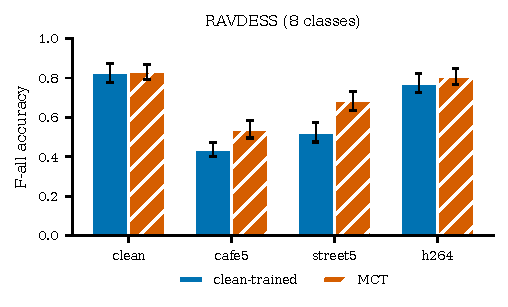
\includegraphics[width=0.6\textwidth]{figures/ext_realistic.pdf}
\caption{F-all accuracy under the realistic degradations for clean-trained and multi-condition-trained models, with 95\% cluster-bootstrap intervals.}\label{fig:realistic}
\end{figure}

\paragraph{Cross-corpus shift.} A change of corpus was the most damaging shift in the study (Table~\ref{tab:cross}, Fig.~\ref{fig:crosscorpus}). Six-class F-all reached 85.8\% within RAVDESS and 79.6\% within CREMA-D. Trained on RAVDESS and tested on CREMA-D it reached 40.6\%, and trained on CREMA-D and tested on RAVDESS 54.9\%. Fusion did not help across corpora: in the CREMA-D-to-RAVDESS direction, CLIP alone (63.5\%) was better than F-all. The fused model's confidence stayed high (0.80 and 0.77), so its ECE rose from about 0.02 to 0.40 and 0.22. Multi-condition training improved F-all across corpora (54.8\% and 60.5\%), which suggests that part of the gap is a channel difference between the recordings. The input monitors noticed the change. Content monitors fitted on RAVDESS flagged 66\% (audio) and 70\% (visual) of clean CREMA-D clips at the per-clip threshold, against about 1\% of held-out RAVDESS clips. The visual quality-descriptor monitor flagged all target clips in both directions, reflecting the different cameras and resolutions. Fitted on RAVDESS, the audio QD monitor flagged only 4\% of CREMA-D clips. Fitted on CREMA-D, the audio content monitor did not distinguish RAVDESS audio (1\% flagged), while the audio quality-descriptor monitor flagged all of it. In every stream that switched from the source to the target corpus, ADWIN raised an alarm and never before the switch. The median delay was 15 clips, except for the audio content monitor fitted on CREMA-D (47 clips).

\begin{table}[t]
\caption{Cross-corpus evaluation on the six shared classes (clean test data). Accuracy with 95\% cluster-bootstrap CI, mean confidence and ECE. Within-corpus rows use subject-independent folds.}\label{tab:cross}
\centering\footnotesize
\begin{tabular}{@{}llrrr@{}}
\toprule
Train $\rightarrow$ test & Model & Accuracy [95\% CI] & Conf. & ECE \\
\midrule
RAVDESS $\rightarrow$ RAVDESS & A1 & 0.758 [0.705, 0.806] & 0.76 & 0.049 \\
 & V1 & 0.704 [0.656, 0.752] & 0.72 & 0.044 \\
 & F-all & 0.858 [0.818, 0.896] & 0.86 & 0.024 \\
CREMA-D $\rightarrow$ RAVDESS & A1 & 0.547 [0.499, 0.594] & 0.68 & 0.132 \\
 & V1 & 0.635 [0.597, 0.673] & 0.69 & 0.069 \\
 & F-all & 0.549 [0.494, 0.606] & 0.77 & 0.221 \\
 & F-all (MCT) & 0.605 [0.546, 0.662] & 0.80 & 0.193 \\
\midrule
CREMA-D $\rightarrow$ CREMA-D & A1 & 0.703 [0.676, 0.732] & 0.72 & 0.027 \\
 & V1 & 0.581 [0.548, 0.612] & 0.60 & 0.030 \\
 & F-all & 0.796 [0.773, 0.821] & 0.79 & 0.019 \\
RAVDESS $\rightarrow$ CREMA-D & A1 & 0.427 [0.405, 0.451] & 0.67 & 0.238 \\
 & V1 & 0.418 [0.388, 0.449] & 0.64 & 0.220 \\
 & F-all & 0.406 [0.376, 0.437] & 0.80 & 0.398 \\
 & F-all (MCT) & 0.548 [0.526, 0.569] & 0.77 & 0.224 \\
\botrule
\end{tabular}
\end{table}

\begin{figure}[t]
\centering
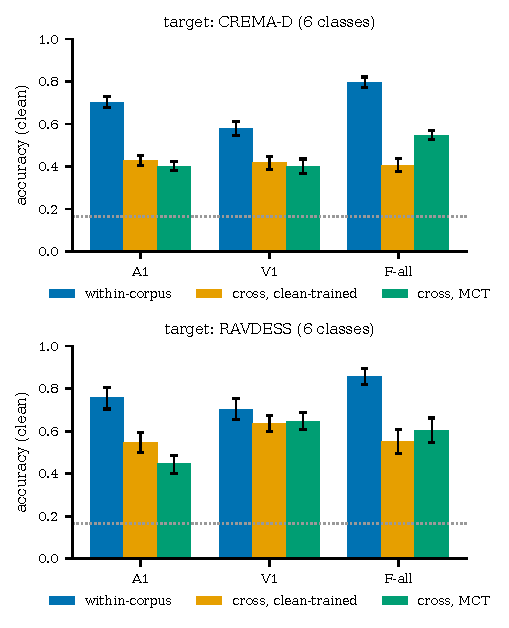
\includegraphics[width=0.6\textwidth]{figures/ext_crosscorpus.pdf}
\caption{Six-class accuracy on clean data within each corpus and across corpora, for models trained on clean data and with multi-condition training. Dashed line: chance.}\label{fig:crosscorpus}
\end{figure}

\paragraph{Monitor variants.} Table~\ref{tab:monitors} compares the monitor variants. On the clean-then-degraded streams (S1), the quality-descriptor (QD) monitors detected every condition on both corpora, typically 16 clips after onset, and attributed each single-channel degradation to the right channel. The content monitors detected H.264 coding in only 48\% of RAVDESS streams and street noise in none of the CREMA-D streams, and they were slower for blur on RAVDESS and for low light, H.264 and cafeteria noise on CREMA-D (median 48 clips). On speaker-blocked clean streams (S4), the QD monitors raised fewer false marks: 12.5\% of RAVDESS streams and 35.0\% of CREMA-D streams had at least one, against 68.3\% and 60.7\% for the content monitors. The reduction was large on RAVDESS and moderate on CREMA-D. (For RAVDESS, the earlier analysis of the same streams reported 69\% and 1.9 marks per 1000 clips. The Cycle~5 re-implementation counts marks slightly differently.) With a degradation starting mid-stream (S5), the QD monitors detected 98.1\% and 97.2\% of degradations against 93.2\% and 86.9\%, with 0.16 and 0.57 false marks per 1000 clips against 1.28 and 1.00. The pre-specified rule therefore selected the QD monitor on RAVDESS, and the choice held on CREMA-D.

The speaker-adaptive monitor raised no false marks, but it detected almost nothing (0.2\% and 0\% of S5 streams). A diagnostic analysis shows why. When a degradation started in the middle of a session, its standardised score rose clearly (mean 2.1 for audio and 4.7 for video on RAVDESS, against 0.1 and 0.7 on clean clips). However, every later session was enrolled on degraded clips, so the normalisation absorbed the degradation, and the mean score fell to 0.2 (audio) and 1.0 (video). In addition, the reset at every session boundary left the detector too few clips to accumulate evidence within one session. The QD+SPK combination therefore behaved like QD alone. Speaker normalisation removes exactly what an input monitor should detect when a degradation lasts longer than a session.

\begin{table}[t]
\setlength{\tabcolsep}{3.5pt}
\caption{Label-free monitor variants. S1: detection rate averaged over degraded conditions; S5: detection rate and median delay (clips) for degradations starting within speaker-blocked streams; S4: false marks per 1000 clips and share of speaker-blocked clean streams with any false mark. RAVDESS: 120 streams per condition; CREMA-D: 140.}\label{tab:monitors}
\centering\footnotesize
\begin{tabular}{@{}llrrrrr@{}}
\toprule
Corpus & Monitor & S1 det. & S5 det. & S5 delay & S4 false/1000 & S4 streams w/ false \\
\midrule
RAVDESS & Content (A0, V0) & 0.953 & 0.932 & 25 & 1.86 & 0.683 \\
 & Quality descriptors & 1.000 & 0.981 & 21 & 0.26 & 0.125 \\
 & Speaker-adaptive & -- & 0.002 & -- & 0.00 & 0.000 \\
\midrule
CREMA-D & Content (A0, V0) & 0.883 & 0.869 & 22 & 1.41 & 0.607 \\
 & Quality descriptors & 1.000 & 0.972 & 21 & 0.80 & 0.350 \\
 & Speaker-adaptive & -- & 0.000 & -- & 0.00 & 0.000 \\
\botrule
\end{tabular}
\end{table}

\begin{figure}[t]
\centering
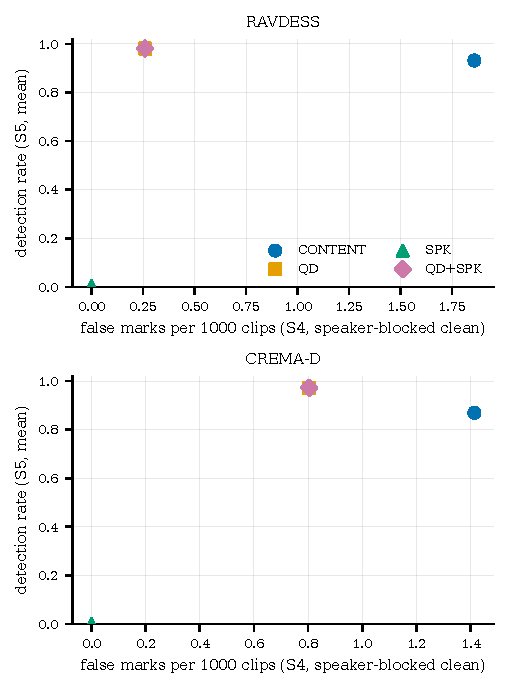
\includegraphics[width=0.55\textwidth]{figures/ext_monitors.pdf}
\caption{Detection rate on streams that degrade within speaker-blocked sessions (S5) against false marks per 1000 clips on speaker-blocked clean streams (S4). Upper left is better. QD+SPK coincides with QD.}\label{fig:monitors-ext}
\end{figure}

\paragraph{Gating with quality-descriptor monitors.} Table~\ref{tab:gating-ext} repeats the gating analysis of Cycles~3 and~4 with the QD monitors on both corpora. For clean-trained models, stream-level gating again recovered most of the accuracy lost to noise (snr10: 37.0\% to 60.6\% on RAVDESS and 35.1\% to 60.2\% on CREMA-D), and it now also helped under the realistic noises (cafe5: 43.6\% to 61.0\% and 48.5\% to 61.2\%). It cost about 6 points under H.264 coding, because the monitor correctly detected a change that the models tolerated, and it then dropped a channel that was still useful. On speaker-blocked clean streams it gated 4.8\% (RAVDESS) and 13.9\% (CREMA-D) of clips and lost 1.1 and 2.0 points. For multi-condition-trained models, envelope-aware gating left the degradations inside the training envelope untouched and helped under cafeteria noise (+5.3 and +7.5 points), but it hurt under street noise ($-$6.2 and $-$8.4 points), where the audio models still added information although the noise lay outside their training envelope: the fused multi-condition model reached 68.3\% and 71.6\%, and dropping audio left 62.1\% and 63.2\%. A monitor that measures how far an input lies from the training data says that the input is new, not that the model fails on it.

\begin{table}[t]
\setlength{\tabcolsep}{4pt}
\caption{Accuracy on the degraded part of S1 streams with QD monitors: clean-trained models without gating (CT) and with stream-level gating (CT+G); multi-condition-trained models without gating (MCT) and with envelope-aware gating (MCT+G). Last rows: accuracy on speaker-blocked clean streams (S4) and share of their clips with a gated channel.}\label{tab:gating-ext}
\centering\footnotesize
\begin{tabular}{@{}lrrrrrrrr@{}}
\toprule
 & \multicolumn{4}{c}{RAVDESS} & \multicolumn{4}{c}{CREMA-D} \\
\cmidrule(lr){2-5}\cmidrule(l){6-9}
Condition & CT & CT+G & MCT & MCT+G & CT & CT+G & MCT & MCT+G \\
\midrule
snr10 & 0.370 & 0.606 & 0.806 & 0.806 & 0.351 & 0.602 & 0.765 & 0.765 \\
snr0 & 0.178 & 0.591 & 0.597 & 0.597 & 0.313 & 0.597 & 0.551 & 0.620 \\
cafe5 & 0.436 & 0.610 & 0.540 & 0.593 & 0.485 & 0.612 & 0.549 & 0.624 \\
street5 & 0.524 & 0.615 & 0.683 & 0.621 & 0.599 & 0.618 & 0.716 & 0.632 \\
compress & 0.702 & 0.708 & 0.803 & 0.803 & 0.653 & 0.697 & 0.741 & 0.741 \\
lowlight & 0.684 & 0.707 & 0.678 & 0.704 & 0.708 & 0.702 & 0.689 & 0.697 \\
h264 & 0.772 & 0.714 & 0.805 & 0.805 & 0.767 & 0.704 & 0.775 & 0.775 \\
\midrule
S4 clean & 0.826 & 0.815 & 0.831 & 0.819 & 0.797 & 0.777 & 0.786 & 0.776 \\
S4 gated share & -- & 4.8\% & -- & 5.7\% & -- & 13.9\% & -- & 10.8\% \\
\botrule
\end{tabular}
\end{table}

\subsection{Spontaneous speech in the wild (Cycle 6)}\label{sec:cycle6}

Cycle~6 applied the design of Cycle~5, with its models, parameters and monitor settings unchanged and the data-specific adaptations of Section~\ref{sec:evaluation}, to 2329 clips of spontaneous speech from 1254 online videos of CMU-MOSEI (Section~\ref{sec:evaluation}). Table~\ref{tab:mosei} summarises the within-corpus results, Fig.~\ref{fig:mosei} the effect of multi-condition training and Fig.~\ref{fig:crosscorpus-mosei} the cross-corpus results.

\begin{table}[t]
\setlength{\tabcolsep}{3.5pt}
\caption{CMU-MOSEI, four classes (2329 clips, 1254 videos, five folds grouped by video; chance 0.25). A1: accuracy and mean confidence of the wav2vec~2.0 stage (clean training). F-all: accuracy of the fused model with clean training (CT) and multi-condition training (MCT). CT+G: clean-trained F-all with stream-level gating on QD monitors, degraded part of S1 streams (the same streams without gating differ from the CT column by at most 0.005). Det.: share of S1 streams in which the QD or CONTENT monitors detected the change (100 streams per condition). $^\dagger$Realistic degradations.}\label{tab:mosei}
\centering\footnotesize
\begin{tabular}{@{}lrrrrrrr@{}}
\toprule
 & \multicolumn{2}{c}{A1 (CT)} & \multicolumn{3}{c}{F-all} & \multicolumn{2}{c}{Det.} \\
\cmidrule(lr){2-3}\cmidrule(lr){4-6}\cmidrule(l){7-8}
Condition & Acc. & Conf. & CT & MCT & CT+G & QD & CONTENT \\
\midrule
clean & 0.498 & 0.475 & 0.558 & 0.557 & -- & -- & -- \\
snr10 & 0.363 & 0.524 & 0.466 & 0.537 & 0.505 & 1.00 & 0.00 \\
snr0 & 0.292 & 0.595 & 0.480 & 0.513 & 0.507 & 1.00 & 0.00 \\
cafe5$^\dagger$ & 0.360 & 0.471 & 0.500 & 0.487 & 0.499 & 0.00 & 0.00 \\
street5$^\dagger$ & 0.402 & 0.461 & 0.532 & 0.521 & 0.530 & 0.00 & 0.00 \\
compress & -- & -- & 0.456 & 0.543 & 0.457 & 0.00 & 0.59 \\
lowlight & -- & -- & 0.490 & 0.484 & 0.495 & 0.87 & 0.30 \\
h264$^\dagger$ & -- & -- & 0.529 & 0.556 & 0.528 & 0.00 & 0.00 \\
snr10+compress & 0.363 & 0.524 & 0.426 & 0.521 & 0.345 & 1.00 & 0.55 \\
snr0+lowlight & 0.292 & 0.595 & 0.406 & 0.420 & 0.381 & 1.00 & 0.31 \\
\botrule
\end{tabular}
\end{table}

\paragraph{Accuracy, fusion and cost.} On clean data F-all reached 55.8\% (macro-F1 0.555) over four classes. This is far below the acted corpora, but well above chance (25\%) and above the best single model, CLIP (50.2\%; gain 5.5 points, 95\% CI [3.0, 8.1], paired cluster bootstrap over videos). wav2vec~2.0 alone reached 49.8\%, and the two cheap models about 44\%. The clips are longer (6.15\,s on average) and half of them have 720p video, so processing costs more than on RAVDESS: F-all needs 5.69\,s per clip (real-time factor 0.93), mostly for CLIP (2.58\,s), wav2vec~2.0 (1.34\,s) and video decoding with face detection (1.28\,s). The A1-first cascade with its threshold fixed on training data escalated 48\% of clips and reached 54.2\% at 3.53\,s per clip, a saving of 38\% for 1.6 points of accuracy.

\paragraph{Silent failure and robust training.} The silent failure replicated. Under 10\,dB white noise, wav2vec~2.0 accuracy fell from 49.8\% to 36.3\% while its mean confidence rose from 0.475 to 0.524, and at 0\,dB accuracy fell to 29.2\% at a confidence of 0.595 (ECE 0.30). The cascade escalated fewer clips under noise (33\% at 10\,dB, 14\% at 0\,dB), and at 0\,dB it reached 31.7\% while F-all reached 48.0\%. With clean training, a degraded channel pulled F-all below the best intact single model under snr10 ($-3.6$ points, CI [$-6.4$, $-0.7$]) and compress ($-4.3$, [$-6.7$, $-1.8$]). Multi-condition training on the same two synthetic degradations as before restored most of this loss (snr10: 46.6\% to 53.7\%; compress: 45.6\% to 54.3\%) without cost on clean data (55.7\%). Unlike on the acted corpora, the realistic noises hurt the clean-trained model only a little ($-5.8$ points for cafeteria and $-2.6$ for street noise, against $-31$ and $-20$ on CREMA-D), and multi-condition training did not help with them.

\paragraph{Monitors in the wild.} Fitted on the training videos, the monitors flagged 0.2--2.4\% of the clean test clips per fold at the P99 threshold, close to the nominal 1\%. The training videos therefore covered the heterogeneity of the test videos. Because a MOSEI stream changes recording every 1.9 clips on average, the clean control streams (S4) contain constant natural variation. Only 2\% (CONTENT) and 3\% (QD) of them had a false mark, far fewer than the speaker-blocked streams of the acted corpora. The flip side was sensitivity. The QD monitors detected white noise in every S1 stream (median delay 16 clips) and low light in 87\%, but they detected neither the realistic noises nor compression nor H.264 coding. The CONTENT monitors detected compression in 59\% and low light in 30\% of streams and no audio degradation at all. A per-clip analysis (Table~\ref{tab:envelope} in the appendix) shows why. On CREMA-D, the audio QD monitor flagged 95\% of cafeteria-noise clips and 86\% of street-noise clips. On MOSEI it flagged fewer than 1\% of the clips under any degradation except 0\,dB white noise, and the video monitors flagged at most 1.0\% under any video degradation. The stream-level detector still caught white noise and low light, because their small shifts of the mean score persisted over many clips, but the realistic noises and the video coding did not shift the scores detectably. This is consistent with the view that recorded noise and low bit rates are already part of the clean reference in online videos, so that a monitor measured against such data sees only shifts beyond this natural range, although we did not test a narrower reference. Most of the degradations that the monitors missed also did little harm to the models (cafe5, street5, h264: $-2.6$ to $-5.8$ points). The exception was compression, which cost the clean-trained model 10.2 points and was seen only by the CONTENT monitor.

\paragraph{Gating.} With clean-trained models, stream-level gating on QD alarms recovered part of the loss under white noise (snr10: 46.6\% to 50.5\%; snr0: 48.0\% to 50.7\%). The recovery was smaller than on the acted corpora; the gated accuracy roughly equalled that of CLIP alone (50.2\%). Gating was harmful when both channels were degraded (snr10+compress: 42.9\% to 34.5\%; snr0+lowlight: 40.1\% to 38.1\%). The audio channel was correctly dropped, but the compressed video that remained was not flagged and carried little information. On clean control streams gating affected 1.5\% of clips and did not change accuracy. With multi-condition training, envelope-aware gating changed accuracy by at most 1.2 points in any condition.

\paragraph{Across corpora.} Models trained on the acted corpora transferred poorly to MOSEI (Fig.~\ref{fig:crosscorpus-mosei}). F-all reached 35.0\% when trained on RAVDESS and 29.8\% when trained on CREMA-D (four classes), against 55.8\% within MOSEI. These models were confidently wrong: mean confidence 0.87 and 0.93, ECE 0.52 and 0.63. Multi-condition training did not change this (37.7\% and 29.4\%). In the other direction, a model trained on MOSEI reached 56.1\% on RAVDESS and 47.5\% on CREMA-D, against 89.1\% and 89.9\% for four-class models trained within these corpora, and it remained calibrated (ECE 0.07 and 0.05). Monitors fitted on an acted corpus flagged 19--100\% of the clean MOSEI clips, depending on monitor and channel, and detected the switch to MOSEI in every stream after 15 clips. Monitors fitted on MOSEI flagged at most 14\% of the acted clips, because the acted recordings lie within the range of the online videos. The QD audio monitor still detected the switch to either acted corpus in every stream (after 15 clips for RAVDESS and 47 for CREMA-D), whereas the CONTENT monitors detected the switch to RAVDESS in only 6\% of streams. A model trained on varied data is harder to surprise, but its monitors are also harder to alarm.

\begin{figure}[t]
\centering
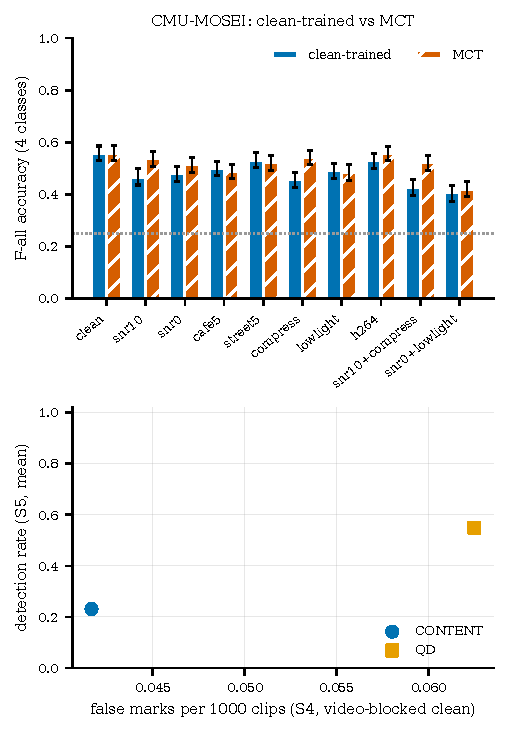
\includegraphics[width=0.62\textwidth]{figures/ext_mosei.pdf}
\caption{CMU-MOSEI. Upper panel: F-all accuracy by condition for clean training and multi-condition training (MCT), with 95\% cluster-bootstrap intervals over videos; dotted line: chance. Lower panel: mean detection rate on S5 streams against false marks per 1000 clips on clean control streams (S4) for the two monitor variants.}\label{fig:mosei}
\end{figure}

\begin{figure}[t]
\centering
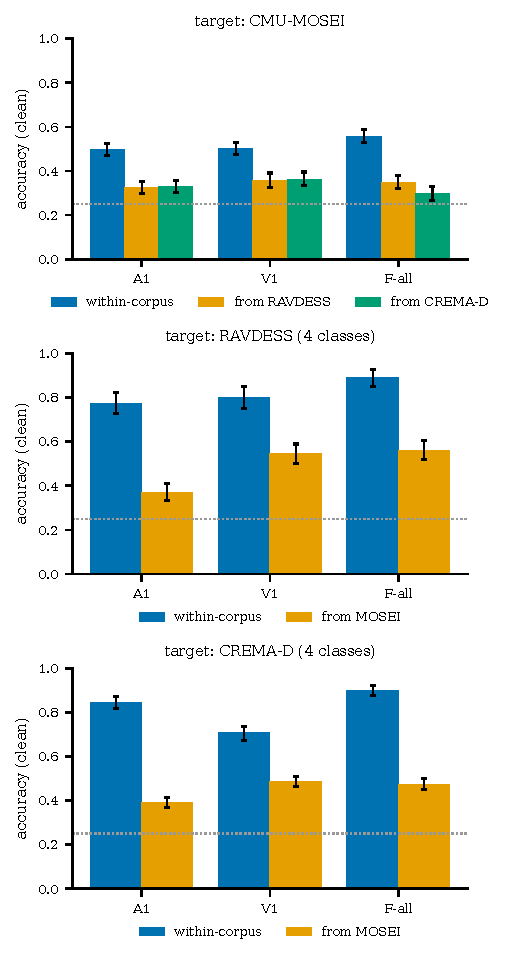
\includegraphics[width=0.5\textwidth]{figures/ext_crosscorpus_mosei.pdf}
\caption{Four-class accuracy on clean data within and across corpora: models tested on CMU-MOSEI (top), and models trained on CMU-MOSEI and tested on RAVDESS (middle) and CREMA-D (bottom). Dotted line: chance.}\label{fig:crosscorpus-mosei}
\end{figure}
